
\documentclass[12pt]{article}
\usepackage{setspace}
\usepackage{tikz}
\usetikzlibrary{arrows}
\usepackage[margin=1in]{geometry}

\begin{document}

\doublespacing

\section{Design}
% An  overview  of  your  complete  system  design,  using  block  diagrams,  pseudocode,  prose,  or  a  mixture  ofsome or all of these.  (This section should focus on the parts of the design that were completed by you, andshould not be a rewording of what is given in the lab manual.)

The music player software is designed in a modular pattern.
The most important sections of these are overviewed below.

The initialization code is run as soon as the board turns on.
It is responsible for running code to initialize the SD card and its FAT file
system, the audio codec, and the button and switch interrupts.
It also reads the SD card, and finds all files with a \texttt{.fat} file
extension, and saves their names and sectors in an array for use later.

Another module is the filesystem related code.
Much of this was provided as part of the lab starter code, although it was also
augmented to be able to treat a file as a stream.
This simplifies the interface exposed to the playback code, which consumes the
data from the file.
% TODO mention bugs in fs code

An interrupt handles the button press, which can change the current song,
playback mode, or playback state (ie: playing/stopped).
Note that because the interrupt handler can only block for a very short period
of time, the handler cannot actually read the next song name off the card.
The initialization process read all of the song files' information into an
array at the start.
The interrupt handler just loops through this array.

The handler propagates changes to the state, mode, or currently selected file
back to the main loop by updating a struct which the interrupt handler and main
loop both have a reference to.
The main loop is responsible for updating the LCD display, because updating it
in the interrupt handler would block for too long.
Primarily, it busy waits until it is signalled to start playing music.

When the playback state changes to start playing a song, the file of whichever
song is currently selected is opened, and a file stream is created.
The audio playback method is passed the filestream, along with a playback mode,
and a reference to the same struct used by the interrupt handler.
The playback method periodically checks the struct, and stops if the playback
mode has changed.
This is used by the interrupt handler to abort playback mid-way through the audio
file.
We can model the state changes as a finite state machine.

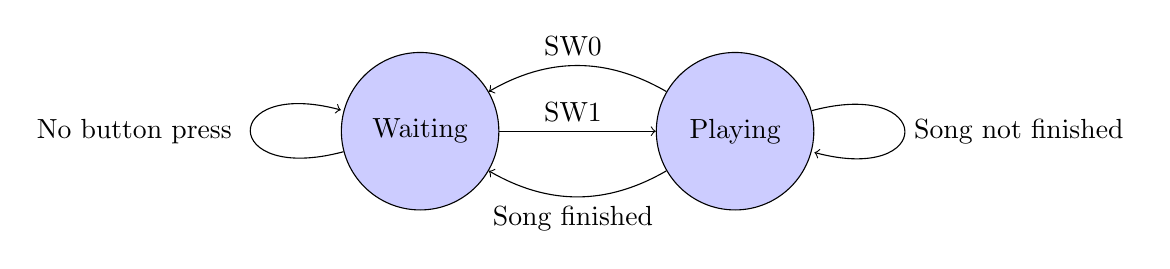
\begin{tikzpicture}[->,node distance=4cm,main/.style={circle,fill=blue!20,draw,minimum size=2cm,align=left}]
    \node[main] (playing) {Playing};
    % \node[main] (start) [below left of=blank] {Start};
    \node[main] (waiting) [left of=playing] {Waiting};
    \path[align=left]
        (playing) edge [bend left] node [below] { Song finished } (waiting)
                  edge [bend right] node [above] { SW0 } (waiting)
                  edge [loop right] node { Song not finished } (playing)
        (waiting) edge node [above] { SW1 } (playing)
                  edge [loop left] node { No button press } (waiting)
    ;
\end{tikzpicture}

\section{Software Interfacing Issues}
% A  discussion  of  the  issues  associated  with  one  aspect  of  your  hardware  design  or  the  software  interfacingpart  of  your  design,  for  example,  the  choice  of  interrupt  priorities  or  issues  with  respect  to  interfacing  tothe buttons, switches or LCD display.
% An indication of one hardware or software interfacing design decision you made given the above issues, andat least one alternative which you discarded.

One of the main problems that we had difficulty with was ensuring that the
left and right audio channels were played on the correct speakers.

The audio device constantly plays audio, consuming audio data from
a FIFO buffer.
The samples are played alternately on the left and right channels of
the audio device.
If the buffer is ever allowed to empty, it implicitly plays a sample with zero
amplitude.
Unfortunately, if a non-deterministic number of samples are consumed from the
buffer, we no longer know whether the next sample enqueued on the buffer will
be played on the left or right channel.
Whenever a blocking operation (usually disk IO) takes too long, the FIFO will
empty, and this bug will be triggered.
There are two specific places where the bug emerges: when reading sectors when
playing double-speed audio, and when reading in the cluster chain of a file.

% TODO diagram?

Essentially, there are two solutions to this problem.
The first possible solution is to never have a blocking operation ``long enough"
to allow the FIFO to empty.
One solution to this issue would be to interleave blocking operations with playing
audio.
Ideally, this would be accomplished with control techniques such as threads, or
coroutines.
This would allow interleaving the computations while still maintaining logically
seperate control flow for the playback and filesystem code.
Unfortunately, coroutines aren't supported by C, and there is no OS on the board
to support threads.

Therefore, the only alternative is to actually mix the filesystem and audio code.
The cluster chain read method would need to be altered to fill up the audio FIFO
with pairs of dummy samples.
A modified \texttt{SD\_read\_lba} method would need to be created, which plays

each 16-bit sample as it is read, instead of buffering the entire sector into
memory.
This kind of code structure would be very poorly structure and modular by its
very definition.
We therefore did not use this solution.

The other possible solution that we could conceive was to allow the FIFO to
empty, but to realize which channel was currently being read in on the device.
We could then resynchronize each time we start playing audio.
If the FIFO is empty, then we would wait until the FIFO is playing a signal on
the left channel, then begin playing music again.
This would still leave some gaps in playback, but would at least maintain
the correct audio channels.
From the datasheet for the audio codec, it appears that such control information
is exposed on the \texttt{DACLCK} line.
Although this value is currently not read, te could create a new parallel IO pin
to read this value, and make it accessible to our software.

Ultimately, we used neither of the solutions mentioned above, because the lab
instructor advised us that fixing this issue was beyond the scope of the lab.

\subsection{Testing \& Debugging}
% A description of the testing and debugging strategy you used for one part of
% your hardware or software interfacing design and at least one alternative
% strategy that you discarded. Indicate any intermediate stages used in your
% design.
For debugging interfacing issues, we initially just used printf.
This technique was quite useful
for determining if a section of code was running at all, i.e. to make sure our
init code was running properly. This came in handy when the board we were
initially using was fried- it would run our code, but get stuck in the SD card
driver initialization, because a input never went low. Quickly isolating the
line that was causing the issue allowed us to switch to another computer and
continue developing the lab. However, this didn't work very effectively when
code was running very quickly- for example, when our sample playing code was
not stopping at the end of a file properly, and would just keep playing
beyond that. Printing inside our sample playing loop would have made the code
run so slowly that we would not have been able to debug it effectively.
Instead, we started displaying the loop counter values on the LEDs. This worked
fairly well, but it was difficult to figure out the value quickly (important
in this case, as the values were changing quickly), and the range of values
that could be displayed was not very big. For these reasons, we eventually
transitioned to using the seven-segment to show values we cared about, in
hexadecimal.

To test audio synchronization, we repeatedly played audio signals with distinct
left and right channels, and checked if the channels changed which speaker they
were playing on over time.
This has the advantage of being a full end-to-end test of the desired
functionality.
In theory, this methodology can only test for the presence of the bug, and not
its absence.
However, when playing at double speed, the channels would switch very frequently,
making this a reliable way to check for this bug.
We would observe the bug immediately when playing at double speed, so if we
did fix the bug, it would be immediately obvious.

Another testing strategy we tried was adding timing logic in the playback code
to find which code was consuming the most amount of time.
This is useful from a debugging perspective, in that it reveals the hotspots in
the code, and allows us to locate long-running, blocking routines that are
triggering the bug.
Unfortunately, adding timing logic adds additional work to the program, which
itself changes the timing of the program.
This created new problems with the playback, such as ``crackly" audio.
For this reason, while this technique gives valuable information, it is not
effective at debugging -- it \emph{creates} bugs.

\section{Playback Performance}
% A discussion of the issues that impacted on the audio playback performance for each of the playback modes.
Normal, reverse, and slow modes played smoothly immediately without additional
code or complexities required, since we had followed the suggestions in the
lab manual of reading the cluster chain beforehand. We were not able to get
double speed mode playing with acceptable performance, because the time spent
reading SD card blocks was simply too long to be able to play every sample on
time. We considered trying to optimize the assembly output for this routine,
in case the compiler was generating suboptimal assembly, but we ran out of
time. We also considered interleaving the SD card code with the audio playing
code (i.e. create a routine which reads 16 bits, plays them, skips 16 bits,
etc, until the end of the file is reached). We thought this could gain some
efficiency because it would not be waiting for the decoder FIFO to have space,
but when we measured, only ~10\% of the time spent playing samples was spent
waiting for the FIFO to have space. Given that the lab manual said double-
speed mode was expected to sound crappy, we stopped working on it at this
point. Delay mode was easy to get "working", but took several iterations to
get acceptable performance and audio quality.

% A discussion of the issues associated with writing effcient software so as to
% meet the performance requirements associated with the system.
% An indication of one software design decision you made given the above two
% performance issues, and at least one alternative which you discarded.
One of the first attempts we made at delay mode simply used two file "streams",
with each reading from different parts of the file. While this was simple and
elegant in code, it did not yield acceptable performance, having many of the
same problems as the double-speed mode, since we were effectively trying to
read twice as many blocks in the same period of time. Thus, despite it's
perfect beauty, we had to discard this technique. The second technique we tried
was to use a ring buffer in order to buffer one second of samples, thus
reducing the number of disk reads to the same as normal speed mode, at the
expense of ram. Initially, this was also much too slow to be workable, until,
after a few hours of debugging, we finally asked a TA for assistance. It turned
out that the CPU we use for this lab does not have a hardware divide module,
so the modulus operation that our ring buffer was using had to be emulated in
software, taking an unacceptably long time.


% A description of the testing and debugging strategy you used for one part of
% your software with regards to the audio playback, and at least one
% alternative strategy that you discarded. Indicate any intermediate stages
% used in your software design.
\subsection{Testing \& Debugging}
In order to debug issues with playback performance, the first strategy we
tried was just randomly changing things. Unsurprisingly, this did not work
particularly well. Debugging issues for audio playback was not easy to do
with our more traditional debugging methods, because often the problem would
not be a logical error in the program, but rather just be
that we were using a technique which was too slow. In order to pinpoint issues
that were contributing to potential slowness, we wrote a stopwatch which used
the 10us onboard timer to allow timing of code sections. This allowed us to
figure out which sections were taking the most time, optimize those sections,
and provided us a way to know if our changes were actually improving the speed
of the relevant code sections- because improvements to the code's speed did
not necessarily lead to perceptible improvements in audio, until we crossed
the threshold of actually being able to play all the samples on time.

% A  brief  discussion  of  a  possible  future  extension  to  the  lab.   Given  more  choice  for  a  final  project  (andpossibly 4-5 weeks in which to do it) and the same equipment, what would you have rather done?
\section{Possible Future Extensions}
There were a few things I would have liked to try as possible future extensions
to this lab:
\begin{enumerate}
\item Show the progress of the current song on the LCD display, or on the LEDs.
\item Make 2x speed actually play the audio properly. This could be pretty
	challenging, but optimizing the raw sd card block reading code could
	probably get pretty far in this direction. We could also increase the
	clock speed of the processor used on the board, or introduce some special-
	purpose instructions for reading the sd card data to allow it to complete
	in fewer clock cycles.
\item Make an equalizer visualization, either on the LCD or the LEDs.
\end{enumerate}

\section{Contribution}
Peter Raboud:
I was responsible for writing most of the playback code (except for the delay mode),
the file stream code, and the button interrupt code.
I also wrote the first half of this report.

The most valuable learning experience from this lab was a practical introduction
in how the FAT file system works.
In previous courses, we usually treat files as a stream.
For efficiency, reads are buffered, but the buffer size can be anything we want.
However, working with the SD card / FAT file system at the low level demonstrates
that files are structured into sectors.
There isn't an efficient way of accessing data in the middle of the sector; that
is, without accessing all of the data before it, and discarding it.
If we want to treat files as streams, we would have to build this functionality
on top of the sector oriented operations supported natively.
The stream-oriented module we wrote kept track of the sectors, how much data was
read, and automatically advanced to the next sector after each read.
However, we only implemented stream oriented methods partially in this lab,
because full support was not required or useful.
We only supported reading exactly one sector at a time, since reading a fraction
of a sector wasn't useful when playing audio.

Justin McGirr:
I was responsible for dissecting the FAT filesystem code to try and figure out
how things worked, writing the timer interfacing code to allow for stopwatch
based debugging, and implementing delay mode. I also wrote the second half of
this report.

The most valuable thing I learned is that the FAT filesystem is quite complex
to work with due to it's legacy and compatibility hacks, despite the fact that
the underlying data structures are very simple (i.e. a singly-linked list).
Reading the provided code to figure out how it works and how to interface with
it was quite challenging as well, because the provided code had some bugs
(which just happen to not matter in the particular filesystem on the provided
SD cards), and because the control flow in many places relied on the use of
global variables rather than function parameters.

I also learned that there exist CPU architectures without hardware divide
(i.e. the CPU we used for this lab), which makes \% (mod) operations very
slow. This caused some significant and hard-to-debug problems when implementing
delay mode, as the ring buffer implementation I wrote made use of the mod
operator extensively when adding and removing data.

\end{document}
